%packages a utilizar:

\setcounter{secnumdepth}{3}
\setcounter{tocdepth}{3}
\setlength{\parskip}{\smallskipamount}
\setlength{\parindent}{0pt}

\documentclass{report}

\usepackage[T1]{fontenc} 

\usepackage[utf8]{inputenc} 

\usepackage[top=3cm,bottom=3cm,left=3cm,right=2.5cm,asymmetric]{geometry} %fronteiras

\usepackage[backend=biber, style=ieee]{biblatex} 

\usepackage{csquotes}

\usepackage[portuguese]{babel} 

\usepackage{blindtext} 

\usepackage[printonlyused]{acronym}

\usepackage{hyperref}

\usepackage{graphicx}

\usepackage{titling}

\usepackage{multicol} %multicoluna de texto

\usepackage{adjustbox}

\renewcommand{\figurename}{Fig.} 

\renewcommand{\tablename}{Tabela} 

\usepackage[font=small,tableposition=top]{caption} 

\usepackage[font=small]{subcaption}

\usepackage{xcolor} %cor nos textos

\usepackage{amsmath} %matematica

\usepackage{amssymb} %simbolos matematicos

\graphicspath{{./imagens/}} %imgs em pasta!

\usepackage{fancyhdr}

\usepackage{authblk}

\usepackage{float}

\usepackage{url} %referencias URL

\usepackage{blindtext}

\def\UrlBreaks{\do\/\do-} %não cortar referencias 
\usepackage{listings}
\usepackage{color}
% Package used for placeholder text
\usepackage{lipsum}

% Prevents LaTeX from filling out a page to the bottom
\raggedbottom
\definecolor{dkgreen}{rgb}{0,0.6,0}
\definecolor{gray}{rgb}{0.5,0.5,0.5}
\definecolor{mauve}{rgb}{0.58,0,0.82}

%code
\lstset{frame=tb,
  language=Java,
  aboveskip=3mm,
  belowskip=3mm,
  showstringspaces=false,
  columns=flexible,
  basicstyle={\small\ttfamily},
  numbers=none,
  numberstyle=\tiny\color{gray},
  keywordstyle=\color{blue},
  commentstyle=\color{dkgreen},
  stringstyle=\color{mauve},
  breaklines=true,
  breakatwhitespace=true,
  tabsize=3
}

\definecolor{mGreen}{rgb}{0,0.6,0}
\definecolor{mGray}{rgb}{0.5,0.5,0.5}
\definecolor{mPurple}{rgb}{0.58,0,0.82}

\lstdefinestyle{C}{
    commentstyle=\color{mGreen},
    keywordstyle=\color{magenta},
    numberstyle=\tiny\color{mGray},
    stringstyle=\color{mPurple},
    basicstyle=\footnotesize,
    breakatwhitespace=false,         
    breaklines=true,                 
    captionpos=b,                    
    keepspaces=true,                 
    numbers=left,                    
    numbersep=5pt,                  
    showspaces=false,                
    showstringspaces=false,
    showtabs=false,                  
    tabsize=2,
    language=C,
    frame=single,
    backgroundcolor=\color{light-gray}
}


\lstdefinestyle{Matlab}{
    commentstyle=\color{mGreen},
    keywordstyle=\color{blue},
    numberstyle=\tiny\color{mGray},
    stringstyle=\color{mGreen},
    basicstyle=\footnotesize,
    breakatwhitespace=false,         
    breaklines=true,                 
    captionpos=b,                    
    keepspaces=true,                 
    numbers=left,                    
    numbersep=5pt,                  
    showspaces=false,                
    showstringspaces=false,
    showtabs=false,                  
    tabsize=2,
    language=Matlab,
    frame=single,
    backgroundcolor=\color{light-gray}
}

\lstdefinestyle{Python}{
   commentstyle=\color{mGreen},
    keywordstyle=\color{magenta},
    numberstyle=\tiny\color{mGray},
    stringstyle=\color{mPurple},
    basicstyle=\footnotesize,
    breakatwhitespace=false,         
    breaklines=true,                 
    captionpos=b,                    
    keepspaces=true,                 
    numbers=left,                    
    numbersep=5pt,                  
    showspaces=false,                
    showstringspaces=false,
    showtabs=false,                  
    tabsize=2,
    language=Python,
    frame=single,
    backgroundcolor=\color{light-gray}
}
%The previous \lstdefinestyle command can be used in the following way:
%\begin{lstlisting}[language = C]
%	
%	\end{lstlisting}

\begin{document}	

	%Capa do Relatório:

\begin{titlepage}
	\clearpage\thispagestyle{empty}
	\centering
	\vspace{2cm}

	
	{\Large Relatório Word Ladder | AED \par}
	\vspace{0.5cm}
	{\small Professores: \\
	Tomás Oliveira e Silva \\
	João Manuel Rodrigues \\
	Joaquim Madeira \\
	Pedro Cirne \\
	Pedro Lavrador\\
	
	\par}
	\vspace{4cm}
	{\Huge \textbf{Word Ladder}} \\
	\vspace{1cm}
	\vspace{4cm}
	{\normalsize Afonso Baixo,108237 - 40\% \\ 
	             Luís Leal, 103511 - 20\% \\ 
	             Paulo Macedo, 102620 - 40\% \par}
	\vspace{2cm}

    
\includegraphics[scale=0.10]{ua.png}
    
    \vspace{2cm}
    
	{\normalsize Departamento de Eletrónica, Telecomunicações e Informática \\ 
		Universidade de Aveiro \par}
		
	{\normalsize 27 dezembro de 2022 \par}
	\vspace{2cm}
	
	\pagebreak

\end{titlepage}


%ÍNDICE:

	\renewcommand{\contentsname}{\'Indice} % name of the indice
	\tableofcontents %indice
	\listoffigures 
	\pagenumbering{roman}

%HEADERS & FOOTERS:

\pagestyle{fancy}
\fancyhf{}
\rhead{\titulo}
\cfoot{\thepage}
\pagenumbering{arabic}

\chapter{Introdução}
\label{introduçao}
\lhead{Introdução}
    Inserido na unidade curricular Algoritmos e Estrutura de Dados, este relatório serve o propósito de analisar e explicar o código produzido para resolver o problema "Word Ladder", proposto pelos professores.
    \\\\
    Este programa tem como objetivo armazenar todas as ligações entre palavras que diferem apenas em uma letra. O objetivo será alcançado através de um grafo composto por vários componentes 
onde cada um armazena as arestas entre as palavras. Com o grafo completo, podemos introduzir uma/duas palavra(s)
e pedir uma das seguintes funções: 
\begin{itemize}
\item Mostrar todas as palavras que se relacionam com a que foi introduzida;
\item Mostrar um caminho, caso ele exista, entre as duas palavras introduzidas.
\end{itemize}

	\section{Pré-requisitos}
	\label{requisitos}
	De forma a compilar o programa, é necessário ter um compilador de C como o gcc instalado na máquina local.
	
	\section{Compilar}
	\label{compilar}
	O seguinte comando permite compilar o programa word ladder (word\_ladder.c):
	\begin{lstlisting}[language=python]
  cc -Wall -Wextra -O2 word_ladder.c -o word_ladder -lm
    \end{lstlisting}
	
	\section{Executar}
	\label{executar}
	Opções:
	\begin{lstlisting}[language=python]
	<wordlist-four-letters.txt> ..... Usa o ficheiro com palavras de 4 letras;
	
	<wordlist-five-letters.txt> ..... Usa o ficheiro com palavras de 5 letras;
	
	<wordlist-six-letters.txt> ...... Usa o ficheiro com palavras de 6 letras;
	
	< > ............................. Usa o ficheiro predefinido(wordlist-big-latest.txt).
	\end{lstlisting}
\pagebreak
	\section{Menu do programa}
	\label{menu}
	Depois de executar ainda existem as seguintes possibilidades:
	\begin{lstlisting}[]
	< 1 > ........................... Encontra o componente conexo da palavra introduzida;
	
	< 2 > ........................... Encontra o caminho entre duas palavras introduzidas;
	
	< 3 > ........................... Termina o programa.
	
	\end{lstlisting}

\chapter{Funções desenvolvidas}
\label{funções}
\lhead{Funções desenvolvidas}
\section{Alocar e libertar memória}
	\begin{lstlisting}[language=C]
static adjacency_node_t *allocate_adjacency_node(void)
{
  adjacency_node_t *node;

  node = (adjacency_node_t *)malloc(sizeof(adjacency_node_t));
  if(node == NULL)
  {
    fprintf(stderr,"allocate_adjacency_node: out of memory\n");
    exit(1);
  }
  return node;
}

static void free_adjacency_node(adjacency_node_t *node)
{
  free(node);
}

static hash_table_node_t *allocate_hash_table_node(void)
{
  hash_table_node_t *node;

  node = (hash_table_node_t *)malloc(sizeof(hash_table_node_t));
  if(node == NULL)
  {
    fprintf(stderr,"allocate_hash_table_node: out of memory\n");
    exit(1);
  }
  return node;
}

static void free_hash_table_node(hash_table_node_t *node)
{
  free(node);
}
    \end{lstlisting}
    \pagebreak
    Para mostrar o funcionamento das funções de alocar e libertar memória foram utilizadas as seguintes \textit{macros}:
    \begin{lstlisting}[language=C]
#define malloc(s) ({void *m = malloc(s); printf("%016lx M %3d %10ld\n",(long)m,__LINE__,(long)(s)); m;})
#define free(s) ({free(s); printf("%016lx F %3d\n",(long)s,__LINE__);})
    \end{lstlisting}
	\section{crc32}
	\label{crc32}
Função usada para atribuir índices (\textit{hashing}) às palavras inseridas na \textit{hash table}.
	\begin{lstlisting}[language=C]
unsigned int crc32(const char *str)
{
  static unsigned int table[256];
  unsigned int crc;

  if(table[1] == 0u) // do we need to initialize the table[] array?
  {
    unsigned int i,j;

    for(i = 0u;i < 256u;i++)
      for(table[i] = i,j = 0u;j < 8u;j++)
        if(table[i] & 1u)
          table[i] = (table[i] >> 1) ^ 0xAED00022u; // "magic" constant
        else
          table[i] >>= 1;
  }
  crc = 0xAED02022u; // initial value (chosen arbitrarily)
  while(*str != '\0')
    crc = (crc >> 8) ^ table[crc & 0xFFu] ^ ((unsigned int)*str++ << 24);
  return crc;
}
	\end{lstlisting}
	
	\section{hash\_table\_create}
	\label{hashtablecreate}
	A função cria uma nova \textit{hash table} que será inicializada com um espaço que corresponde a 100 elementos do \textit{array heads} e o número de entradas e de vértices será inicializado com o valor 0. Cada posição da tabela representa um ponteiro para uma \textit{linked list} na qual, posteriormente, serão armazenadas as palavras. O array de ponteiros \textit{heads} contém o ponteiro para a \textit{head} de cada lista e este aponta inicialmente para NULL.
	
	\begin{lstlisting}[language=C]
static hash_table_t *hash_table_create(void)
{
  hash_table_t *hash_table;
  unsigned int i;

  hash_table = (hash_table_t *)malloc(sizeof(hash_table_t));
  if(hash_table == NULL)
  {
    fprintf(stderr,"create_hash_table: out of memory\n");
    exit(1);
  }
  hash_table->hash_table_size = 100; //initial size of the hash table
  hash_table->number_of_entries = 0;
  hash_table->number_of_edges = 0;
~  hash_table->heads = (hash_table_node_t **)malloc(sizeof(hash_table_node_t) * hash_table->hash_table_size);
  if(hash_table->heads == NULL){
    fprintf(stderr,"hash_table_table: out of memory\n");
    exit(1);
 ´  }
  for(i = 0; i < hash_table->hash_table_size; i++){
    hash_table->heads[i] = NULL;
  }
  printf("hash table created (size: %d)\n",hash_table->hash_table_size);
  return hash_table;
}
	\end{lstlisting}
	
	\section{hash\_table\_free}
	\label{hashtablefree}
	A função serve o propósito de libertar a memória alocada préviamente para a \textit{hash table} e fá-lo-á percorrendo primeiramente o \texti{array} de ponteiros \textif{heads} onde cada ponteiro irá apontar para as \textit{linked lists}. Por cada nó pertencente a uma \textit{linked list}, antes de este ser libertado, é percorrida a sua lista de adjacência e, após serem libertadas todas as suas adjacências, o processo prossegue para o nó seguinte. Após os nós serem todos libertados, será libertado o \textit{array} de ponteiros \textit{heads} e, por último, a \textit{hash table}.

	\begin{lstlisting}[language=C]
static void hash_table_free(hash_table_t *hash_table)
{
  if(hash_table == NULL)
    return;
  for (unsigned int i = 0; i < hash_table->hash_table_size; i++)
  {
    hash_table_node_t *entry = hash_table->heads[i];
    while(entry != NULL){
      hash_table_node_t *last_entry = entry;
      adjacency_node_t *adjacency_node = entry->head;
      while(adjacency_node != NULL){
        adjacency_node_t *last_adjacency = adjacency_node;
        adjacency_node = last_adjacency->next;
        free_adjacency_node(last_adjacency);
      }
      entry = last_entry->next;
      free_hash_table_node(last_entry); 
    }
  }
  free(hash_table->heads);
  free(hash_table);
}	
	\end{lstlisting}
	
	\section{hash\_table\_grow}
	\label{hashtablegrow}
A função \textit{hash\_table\_grow} tems como objetivo aumentar o tamanho da \textit{hash table} original. Este processo passa por criar uma nova \textit{hash table} com o dobro do tamanho da original e, percorrendo todos os nós e todas as palavras da tabela anterior e com recurso à função crc32 (\ref{crc32}), serão calculados novos índices para as palavras armazenadas na tabela antiga, de forma a que possam ser corretamente armazenadas na nova tabela. As posições da tabela são todas inicializadas com um ponteiro nulo.
\\
Quando este processo termina, a memória alocada para a tabela antiga é libertada, o \textit{array heads} corresponderá ao \textit{array new\_heads}, que possui os nós atualizados e o valor da variável \textit{hash\_table\_size} também é atualizado para o novo tamanho da \textit{hash table}.\\

	\begin{lstlisting}[language=C]
static void hash_table_grow(hash_table_t *hash_table)
{
  unsigned int new_size = hash_table->hash_table_size * 2;
  // Create a new hash table 
  hash_table_node_t **new_heads = (hash_table_node_t **)malloc(sizeof(hash_table_node_t) * new_size);
  if(new_heads == NULL) exit(1);

  // Initialize new hash table
  for (unsigned int i = 0; i < new_size; i++)
    new_heads[i] = NULL;

  for(unsigned int i = 0; i < hash_table->hash_table_size; i++){
    hash_table_node_t *entry = hash_table->heads[i];
    while(entry != NULL){
      //Insert node into the new hash table
      hash_table_node_t *last_entry = entry;
      unsigned int new_index = crc32(entry->word) % new_size;
      if(new_heads[new_index] == NULL){
        new_heads[new_index] = entry;
      } else {
        hash_table_node_t *current = new_heads[new_index];
        while(current->next != NULL)
          current = current->next;
        current->next = entry;
      }
      entry = entry->next;
      last_entry->next = NULL; 
    }
  }
  //Free the old hash table and assign the new one
  free(hash_table->heads);
  hash_table->heads = new_heads;
  hash_table->hash_table_size = new_size;
  printf("hash table resized (new size: %d, entries: %d)\n", new_size, hash_table->number_of_entries);
}
	\end{lstlisting}
	
	\section{find\_word}
	\label{findword}
Esta função tem como objetivo principal encontrar uma palavra que será passada nos parâmetros de entrada e devolver o nó onde se encontra. Caso a palavra não esteja na \textit{hash\_table}, será adicionada à mesma.\\
	Em primeiro lugar, com recurso à função crc32 (\ref{crc32}), será calculado o índice da palavra a encontrar e, de seguida, será procurado no \textit{array} de ponteiros \textit{heads}, o ponteiro que aponta para a \textit{linked list} onde poderá estar armazenada a palavra. Os nós da lista são percorridos e a palavra armazenada em cada nó é comparada com a palavra a encontrar. Caso a palavra seja encontrada, o ponteiro para o nó onde esta se encontra é devolvido. Caso contrário, será necessário adicionar a palavra à tabela. Para isso, é verificado se o número de elementos da \textit{hash table} é superior a 60\% do seu tamanho total e, caso se verifique, é chamada a \textit{função hash\_table\_grow} (\ref{hashtablegrow}), para aumentar o tamanho da tabela e, por fim, inserir a palavra.
	
	\begin{lstlisting}[language=C]
static hash_table_node_t *find_word(hash_table_t *hash_table,const char *word,int insert_if_not_found)
{
  hash_table_node_t *node;
  unsigned int i;

  i = crc32(word) % hash_table->hash_table_size;
  //Find the node 
  node = hash_table->heads[i];
  while (node != NULL)
  {
    if(strcmp(node->word,word) == 0)
      break;
    node = node->next;
  }
  //If the node wasn't found and we must insert it
  if(node == NULL && insert_if_not_found)
  {
    if((unsigned int)(hash_table->hash_table_size * 0.6) <= hash_table->number_of_entries)
      hash_table_grow(hash_table);
    node = allocate_hash_table_node();
    if(node == NULL) exit(1);
    strcpy(node->word, word);
    // Node values
    node->next = NULL;
    node->previous = NULL;
    node->representative = node;
    node->number_of_edges = 0;
    node->number_of_vertices = 1;
    node->visited = 0;
    node->head = NULL;
    //Insert the node into the linked list at the hash index
    if(hash_table->heads[i] == NULL){
      hash_table->heads[i] = node;
    } else {
      hash_table_node_t *current = hash_table->heads[i];
      while (current->next != NULL)
      {
        current = current->next;
      }
      current->next = node;
    }
    hash_table->number_of_entries += 1;
  }
  
  return node;
}
	\end{lstlisting}
	
	\section{find\_representative}
Cada nó tem um ponteiro representante que é inicializado apontando para si mesmo.
Quando um nó é adicionado a um componente, as palavras desse componente passam a ter 
um novo representante que será aquele que foi adicionado. Desta maneira, a procura será feita 
passando pelo ciclo que procurará o seu representante. Este ciclo irá parar 
quando o representante de um certo nó for ele mesmo. Neste caso, sabe-se que 
esse será o representante atual. Num novo ciclo, são percorridos todos os nós que foram iterados e 
assimilado o seu representante ao representante do componente atual.
	
	\label{findrepresentative}
	\begin{lstlisting}[language=C]
static hash_table_node_t *find_representative(hash_table_node_t *node)
{
  hash_table_node_t *representative,*next_node,*n;
  for(representative = node;representative->representative != representative; representative = representative->representative)
  ;
  for(n = node; n != representative; n = next_node){
    next_node = n->representative;
    n->representative = representative;
  }
  return representative;
}
	\end{lstlisting}
	
	\section{add\_edge}
Nesta função são considerados dois passos importantes.
A associação de palavras adjacentes (\textit{link} e \textit{link2}), e o novo valor da quantidade de edges e vértices.
Para o primeiro passo, são alocados dois \textit{hash\_table\_node\_t}. Percorrendo os nós adjacentes 
a uma palavra, é verificada se a nova adjacência já existe e, se não existir, são colocados o \textit{link} e \textit{link2} no início
da lista de adjacência das respetivas palavras '\textit{from}' e '\textit{to}'.
Já para o segundo passo, temos de verificar se as palavras pertencem ao mesmo grafo utilizando a função \textit{find\_representative} (\ref{findrepresentative}).
Se pertencerem o resultado será apenas incrementado no valor de \textit{edges} do componente, caso contrário, o resultado será a união dos dois componentes, obtendo como novo valor de vértices, a soma 
dos vertices dos dois componentes, e como valor de edges, a soma de edges dos dois componentes mais o incremento de um (que será a \textit{edge} que foi criada).
	
	\label{addedge}
	\begin{lstlisting}[language=C]
static void add_edge(hash_table_t *hash_table,hash_table_node_t *from,const char *word)
{
  hash_table_node_t *to,*from_rep,*to_rep;
  adjacency_node_t *link;
  to = find_word(hash_table,word,0);
  if(to == NULL)
    return;
  // find the representative of the two nodes
  from_rep = find_representative(from);
  to_rep = find_representative(to);

  // add the edge between the two nodes 
  for(link = from->head; link != NULL && link->vertex != to; link = link->next)
    ;
  if(link != NULL)   // If adjacency is already registered, return
    return;
  link = allocate_adjacency_node();
  link->next = from->head;
  from->head = link;
  link->vertex = to;
  adjacency_node_t *link2; // Add a link in 'node to' as well
  for(link2 = to->head; link2 != NULL && link2->vertex != from; link2 = link2->next)
    ;
  link2 = allocate_adjacency_node();
  link2->next = to->head;
  to->head = link2;
  link2->vertex = from;
    

  // if the representatives are not the same, make one representative of the other
  if(from_rep != to_rep)
  {
    if(from_rep->number_of_vertices >= to_rep->number_of_vertices){
      to_rep->number_of_vertices += from_rep->number_of_vertices;
      to_rep->number_of_edges += from_rep->number_of_edges + 1;  
      from_rep->representative = to_rep;
    } else {
      from_rep->number_of_vertices += to_rep->number_of_vertices;
      from_rep->number_of_edges += to_rep->number_of_edges + 1;
      to_rep->representative = from_rep;
    }
  }
  else
  {
    from_rep->number_of_edges += 1;
  }
  hash_table->number_of_edges += 1;
}
	\end{lstlisting}
	
	\section{breadth\_first\_search}
	\label{breadthfirstsearch}
A inicialização desta função é pensada antes da chamada à função para ter em conta o espaço
necessário a ser alocado para a \textit{list\_of\_vertices}. Após a chamada, esta lista será inicializada
com o nó '\textit{origin}' no índice '0' e as variáveis do tipo inteiro \textit{read} e \textit{write}, com os valores '0' e '1', respetivamente.
É percorrida a lista de adjacência do nó e, se o vértice dessa adjacência ainda não tiver sido visitado,
é marcado como visitado, adicionado à \textit{list\_of\_vertices} e guardado o pai no ponteiro \textit{previous}, deste modo, serão percorridos os seguintes 
elementos que estejam na \textit{list\_of\_vertices}, até um dos seguintes casos acontecer:
\begin{enumerate}
\item O vértice que está a ser visitado corresponde ao nó \textit{goal};
\item Os nós e as respetivas adjacências foram todos percorridos mas o nó \textit{goal} não foi encontrado.
\end{enumerate}
Após um dos casos supra-mencionados acontecer e, percorridos novamente os nós que foram previamente marcados com o auxílio do ponteiro \textit{previous}, 
é colocado o seu valor como não visitado, para possibilitar uma pesquisa futura. Para finalizar, definine-se o índice seguinte da \textit{list\_of\_vertices} como NULL,
para facilicar uma possível pesquisa nessa lista fora da função.
(Note-se que há um caso extra. Este será descrito na função \textit{connected\_component\_diameter} (\ref{connectedcomponentdiameter}),visto que é um caso especial
apenas utilizado nesta função).

	\begin{lstlisting}[language=C]
static int breadth_first_search(hash_table_node_t **list_of_vertices,hash_table_node_t *origin,hash_table_node_t *goal){
  int r = 0;
  int w = 1;
  list_of_vertices[0] = origin;
  origin->visited = 1;
  int distance = 0;
  hash_table_node_t *n;
  adjacency_node_t *nn;
  hash_table_node_t *last_node = NULL;
  while (r < w)
  {
    n = list_of_vertices[r++];
    for (nn = n->head; nn != NULL; nn = nn->next)
    {
      if (nn->vertex->visited == 0)
      {
        list_of_vertices[w++] = nn->vertex;
        nn->vertex->visited = 1;
        nn->vertex->previous = n;
        if (nn->vertex == goal)
        {
          list_of_vertices[w] = NULL;
          for (n = list_of_vertices[0], r = 1; r != w + 1; n = list_of_vertices[r++])
          {
            n->visited = 0;
          }
          return 0;
        }
        last_node = nn->vertex;
      }
    }
  }
  list_of_vertices[w] = NULL;
  for (n = list_of_vertices[0], r = 1; r != w + 1; n = list_of_vertices[r++])
  {
    n->visited = 0;
  }
  if (goal == NULL)
  {
    list_of_vertices[0] = last_node;
    if (last_node != NULL){
      for(; last_node != origin; last_node = last_node->previous)
        distance++;
    }
    return distance;
  }
  return -1;
}
	\end{lstlisting}
	
	\section{list\_connected\_component}
	\label{listconnectedcomponent}
Dada uma palavra, é encontrado o seu respetivo nó utilizando a função \textit{find\_word} (\ref{findword}), é verificada a sua existência,
e prossegue-se guardando o seu representante. Utilizando a função \textit{breadth\_first\_search} (\ref{breadthfirstsearch}), com destino a NULL é percorrido o componente inteiro da palavra que foi dada e os respetivos nós dos componentes serão guardados na \textit{list\_of\_vertices}. Com esta lista basta percorrer todos os índices até o valor de um deles ser NULL.

	\begin{lstlisting}[language=C]
	static void list_connected_component(hash_table_t *hash_table,const char *word)
{
  // Get the vertex corresponding to the given word
  hash_table_node_t *vertex = find_word(hash_table,word,0);
  if(vertex == NULL)
    return;
  // Get the representative of the connected component
  hash_table_node_t *representative = find_representative(vertex);
  if(representative == NULL)
    return;
  int count = 1;
  int component_vertices = representative->number_of_vertices;
  hash_table_node_t **list_vertices = (hash_table_node_t**)malloc(sizeof(hash_table_node_t) * component_vertices);
  breadth_first_search(list_vertices, vertex, NULL);
  printf("%s\n", vertex->word);
  for(hash_table_node_t *node = list_vertices[1]; node != NULL; node = list_vertices[count]){
    printf("%s\n", node->word);
    count++;
  }
  free(list_vertices);
  printf("Component vertices: %d\n", representative->number_of_vertices);
  printf("Component edges: %d\n", representative->number_of_edges);
}
	\end{lstlisting}
	
	\section{path\_finder}
	\label{pathfinder}
Da mesma forma que na função \textit{list\_connected\_component} (\ref{listconnectedcomponent}), são procurados os nós das palavras fornecidas, mas, neste caso, pretende-se mostrar o caminho entre duas palavras. Para isso, será novamente utilizada a função \textit{breadth\_first\_search} 
que, neste caso, terá como \textit{origin} a palavra '\textit{from}' e como \textit{goal} a palavra '\textit{to}'. Deste modo, se tudo correr bem, o valor retornado 
será diferente de '-1' e, nesse caso, depreende-se que a partir da palavra '\textit{to}' existirá um caminho até à '\textit{from}'.
Assim, basta percorrer todos os ponteiros \textit{previous} até que este seja igual ao nó '\textit{to}'.	

	\begin{lstlisting}[language=C]

static void path_finder(hash_table_t *hash_table,const char *from_word,const char *to_word)
{
  hash_table_node_t *nn;
  hash_table_node_t *from = find_word(hash_table,from_word,0);
  hash_table_node_t *to = find_word(hash_table,to_word,0);
  if(from == NULL || to == NULL) return;
  int component_vertices = find_representative(from)->number_of_vertices;
  hash_table_node_t **list_of_vertices = (hash_table_node_t **)malloc(sizeof(hash_table_node_t) * component_vertices);
  if (breadth_first_search(list_of_vertices,from,to) == -1){
    printf("There's no path!\n");
  } else {
    int i = 0;
    hash_table_node_t *last_node = NULL;
    from->previous = NULL;
    for(hash_table_node_t *n = to; n != NULL; n = nn){
      nn = n->previous;
      n->previous = last_node;
      last_node = n;
    }
    for(hash_table_node_t *n = from; n != to; n = n->previous)
      printf("[%2d] %s\n",i++,n->word);
    printf("[%2d] %s\n", i, to->word);
  }
  free(list_of_vertices);
}
	\end{lstlisting}
	
	\section{connected\_component\_diameter}
	\label{connectedcomponentdiameter}
Esta função tem o auxílio de um caso especial na função \textit{breadh\_first\_search} (\ref{breadthfirstsearch}), de modo a aumentar a eficiência
da mesma. Em primeiro lugar, a ideia será guardar todos os nós pertencentes ao componente fornecido.
Posteriomente, serão iteradas todas as adjacências com o \textit{breadh\_first\_search} (\ref{breadthfirstsearch}), com destino a NULL, e é guardado o último nó visitado 
numa variável \textit{last\_node}. Com o auxílio desta variável, são percorridos todos os ponteiros \textit{previous} até encontrar o nó \textit{origin}, incrementando 
sempre no valor da variável \textit{distance} que, futuramente, será retornada pela função. Após executar este processo para todos os nós da lista, é guardada a maior distância de entre todas as distâncias mais pequenas retornadas, obtendo assim o diâmetro do componente.
Esta será toda a essência desta função. Mas, como se pode notar, é feita uma pequena alteração que permite mostrar o caminho entre 2 palavras
que tenham a mesma distância que o argumento de entrada \textit{print\_this\_diameter}, utilizando a função \textit{path\_finder} (\ref{pathfinder}) e o auxílio do caso especial da função \textit{breadh\_first\_search} (\ref{breadthfirstsearch}), que 
guarda o valor da última palavra no índice '0' da lista \textit{list\_of\_vertices}.	
	
	\begin{lstlisting}[language=C]
static int connected_component_diameter(hash_table_t *hash_table, hash_table_node_t *node, int print_this_diameter)
{
  if(node == NULL) return -1;
  int diameter = 0,component_diameter = 0;
  int i = 1;
  int component_vertices = find_representative(node)->number_of_vertices;
  hash_table_node_t **list_of_component_vertices = (hash_table_node_t **)malloc(sizeof(hash_table_node_t) * component_vertices);
  breadth_first_search(list_of_component_vertices,node,NULL); // The first breadth first search that will save all vertices on list_of_vertices
  for(; list_of_component_vertices[i] != NULL && i<component_vertices; i++){
    hash_table_node_t **list_of_vertices = (hash_table_node_t **)malloc(sizeof(hash_table_node_t) * component_vertices);
    node = list_of_component_vertices[i];
    diameter = breadth_first_search(list_of_vertices, node, NULL);
    if(diameter == print_this_diameter){
      path_finder(hash_table, node->word, list_of_vertices[0]->word);
      print_this_diameter = -1;
    }
    if(diameter > component_diameter && diameter >= 0){ 
      component_diameter = diameter;
    }
    free(list_of_vertices);
  }
  free(list_of_component_vertices);

  return component_diameter;
}
	\end{lstlisting}
	\section{graph\_info}
	\label{graphinfo}
Como o próprio nome indica, o objetivo será mostrar informações interessantes do grafo que foi construído.
Para isso, foi decidido mostrar o número de componentes de cada diâmetro encontrado no grafo e é armazenado o maior diâmetro na variável \textit{largest\_diameter}.
O \textit{largest\_diameter} com o seu nó guardado na variável \textit{largest\_diameter\_node}, será utilizado novamente, para mostrar
o caminho mais longo que existe neste grafo.
Para alcançar estes objetivos, é inicilizada uma lista (\textit{list\_of\_components}) onde serão guardados os representantes de todos os componentes, 
que será feito a partir da iteração de todos os nós da \textit{hash\_table}, e verificando se o seu representante já se encontra na lista, caso contrário, este será adicionado.
Com a lista completa, pode-se finalmente percorrer e calcular o diâmetro de todos os nós desta lista (que representam componentes diferentes) obtendo os valores do número de diferentes diâmetros e guardando o valor do nó com o diâmetro mais alto, para depois ser utilizado e, posteriormente, mostrar esse caminho.

	\begin{lstlisting}[language=C]
static void graph_info(hash_table_t *hash_table)
{
  int j;
  int diameter;
  int largest_diameter_count = 0, largest_diameter = 0, num_of_components = 0;
  hash_table_node_t *largest_diameter_node = NULL;
  hash_table_node_t **list_of_components = (hash_table_node_t **)malloc(sizeof(hash_table_node_t) * (hash_table->hash_table_size)/2);
  hash_table_node_t *entry = NULL;
  for(unsigned int i = 0; i < hash_table->hash_table_size; i++){
    entry = hash_table->heads[i];
    while (entry != NULL)
    {
      hash_table_node_t *representative = find_representative(entry);
      for(j = 0; j < num_of_components && representative != list_of_components[j]; j++)
        ;
      if(j == num_of_components) list_of_components[num_of_components++] = representative;
      entry = entry->next;
    }
  }
  int store_diameters[1000] = {0};
  j= 1;
  for(hash_table_node_t *node = list_of_components[0] ; j < num_of_components; node = list_of_components[j++]){
    diameter = connected_component_diameter(hash_table, node, -1);
    if(diameter >= 0) store_diameters[diameter]++;
    if (diameter == largest_diameter) largest_diameter_count++;
    if(diameter > largest_diameter){
      largest_diameter_count = 1;
      largest_diameter = diameter;
      largest_diameter_node = node;
    }
  }
  free(list_of_components);
  printf("%d vertices\n",hash_table->number_of_entries);
  printf("%d edges\n", hash_table->number_of_edges);
  printf("%d connected components\n",num_of_components);
  printf("Number of connected components with a diameter of:\n");
  for(j = 0; j<=largest_diameter; j++){
    if(store_diameters[j] != 0) 
      printf(" %d: %d\n", j, store_diameters[j]);
  }
  printf("largest word ladder:\n");
  connected_component_diameter(hash_table, largest_diameter_node, largest_diameter);
}
	\end{lstlisting}
	\section{show\_all\_paths}
	\label{showallpaths}
	Esta função foi uma implementação extra com intuito de mostrar todas as arestas de todas as palavras pertencentes a um componente, relacionando-as um a um (palavra -> {arestas}).
Para alcançar este objetivo, é feita a utilização de um ficheiro de texto onde serão guardados os valores pretendidos.
É feita a passagem da palavra introduzida onde se irá buscar o nó, através da função \textit{find\_word}. A partir daí, são guardados numa lista todos os nós pertencentes ao componente com o auxílio da função \textit{breadth\_first\_search} (\ref{breadthfirstsearch}) que, mais tarde, serão percorridos um a um e será feita a iteração das suas adjacências para 
serem armazenadas no ficheiro de texto com a ligação da palavra principal respetiva.\\
	\begin{lstlisting}[language=C]
static void show_all_paths(hash_table_t *hash_table, const char *word){
  int i = 1;
  hash_table_node_t *node = find_word(hash_table, word, 0);
  if(node == NULL) return;
  FILE *f = fopen("all_connections.txt", "w");
  adjacency_node_t *n = node->head;
  fprintf(f, "%s->{%s", node->word, n->vertex->word);
  n = n->next;
  while(n != NULL){
    fprintf(f, ", %s", n->vertex->word);
    n = n->next;
  }
  fprintf(f, "}\n\n");
  int component_vertices = find_representative(node)->number_of_vertices;
  hash_table_node_t **list_of_component_vertices = (hash_table_node_t**)malloc(sizeof(hash_table_node_t) * component_vertices);
  breadth_first_search(list_of_component_vertices,node, NULL); 
  for(; list_of_component_vertices[i] != NULL && i<component_vertices; i++){
    n = list_of_component_vertices[i]->head;
    fprintf(f, "%s->{%s", list_of_component_vertices[i]->word, n->vertex->word);
    n = n->next;
    while(n != NULL){
      fprintf(f, ", %s", n->vertex->word);
      n = n->next;
    }
    fprintf(f, "}\n\n");
  }
  free(list_of_component_vertices);
  fclose(f);
}
	\end{lstlisting}
	Esta função é depois adicionada à função \textit{main}, acrescentando mais uma opção no \textit{menu} do programa, com o seguinte formato:
	\begin{lstlisting}[language=C]
else if(command == 4){
      if(scanf("%99s",word) != 1) break;
      show_all_paths(hash_table, word);
    }
	\end{lstlisting}
\chapter{Resultados}
\label{resultados}
De forma a transformar alguns dados obtidos num histograma, foi utilizado um programa \textit{MATLAB}.\\
O excerto de código que se segue é um exemplo de um programa em \textit{MATLAB} para gerar o histograma com dados da \textit{hash table}.
	\begin{lstlisting}[language=Matlab]
clear;
clc;

h = load("histograma.txt");
hf = figure();
entries = h(:,2);
plot(2,1,1);
a = bar(entries,'k');
legend(a,{'Nº de entradas'});
title("Distribuicao das entradas da Hash Table");

print(hf, "hash_table_entries", "-dpdflatexstandalone");
system ("pdflatex hash_table_entries");
open hash_table_entries.pdf
	\end{lstlisting}
\pagebreak
	\section{Dados da Hash Table}
	Nas seguintes demonstrações, por razões de simplicidade, vai ser utilizado o ficheiro \verb|<wordlist-four-letters.txt>| \ref{executar}.\\\\
	\begin{figure}[h!]
    \centering
    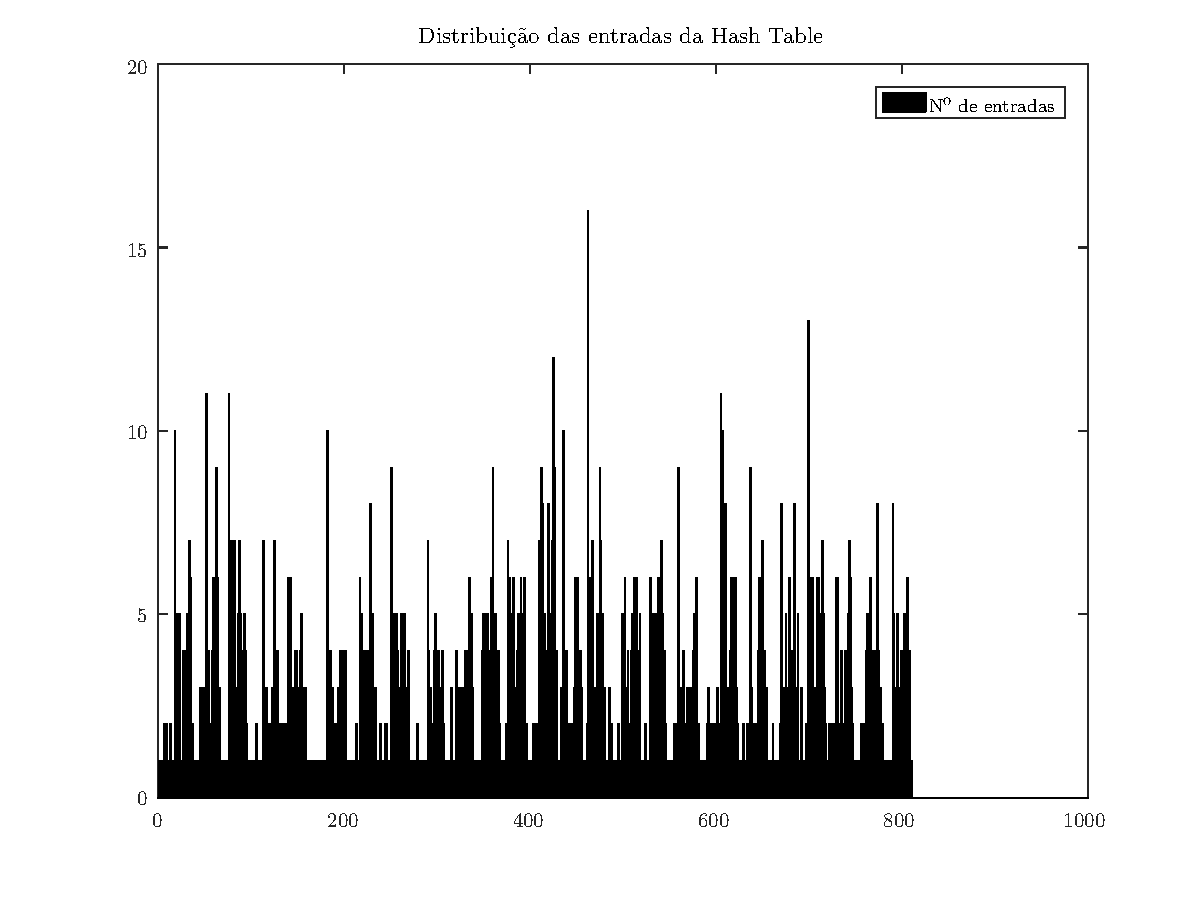
\includegraphics[scale=0.60]{hash_table_entries.pdf}
    \caption{Distribuição das entradas da \textit{hash table}.}
	\end{figure}\\\\
	O histograma visa demonstrar o espaçamento entre as palavras introduzidas na indexação da hash\_table. Isto servirá para perceber (graficamente) se existem zonas mais densas do que outras ou se a inserção está bem distribuída.
\pagebreak
	\begin{figure}[h!]
    \centering
    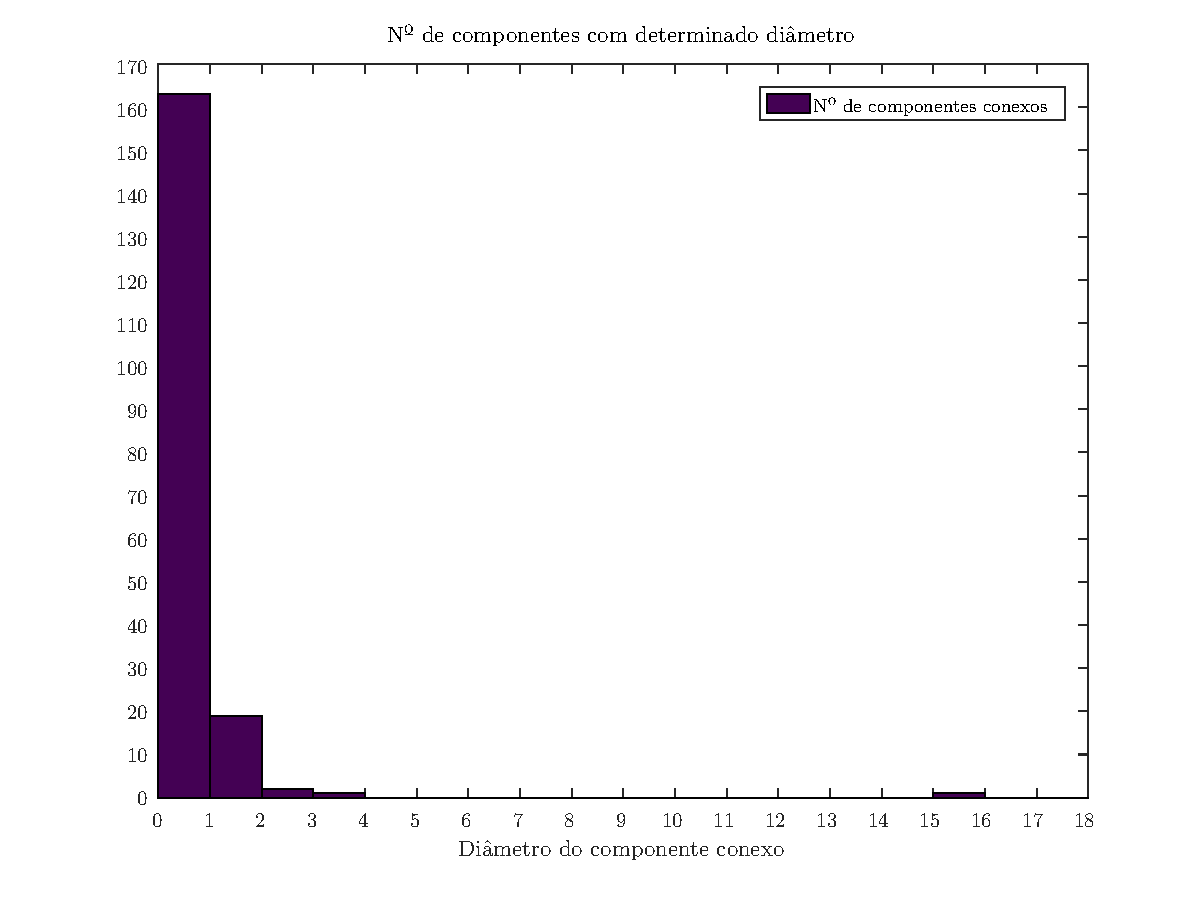
\includegraphics[scale=0.60]{diamComponenteconexo.pdf}
    \caption{Diâmetro dos vários componentes conexos da hash table.}
	\end{figure}\\\\
O histograma visa demonstrar a \textit{ratio} entre um certo diâmetro e o número de componentes cujo diâmetro é esse valor.\\\\
	
	\begin{figure}[h!]
    \centering
    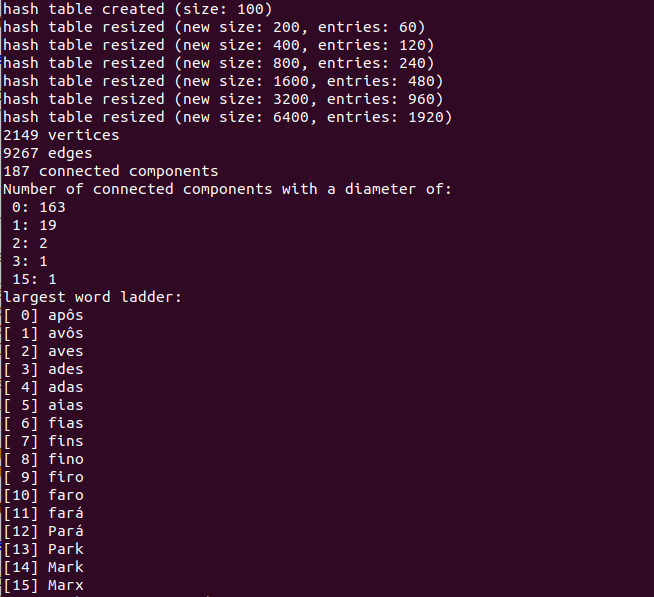
\includegraphics[scale=0.40]{output.png}
    \caption{Demonstração do \textit{output} da função \textit{graph\_info}\ref{graphinfo}.}
    \label{fig:output}
	\end{figure}\\\\
\pagebreak
Para mostrar a informação proveniente da função \textit{grap\_info} \ref{graphinfo}, foi usado, o ficheiro \verb|<wordlist-four-letters.txt>| \ref{executar}. Na Figura~\ref{fig:output}, é possível observar várias informações, não só da \textit{hash table} mas também dos componentes conexos que nela existem, tais como:
\begin{itemize}
\item Criação e redimensionamento da hash table;
\item Nº de vértices e arestas;
\item Nº de componentes conexos;
\item Nº de componentes conexos com um determinado diâmetro;
\item O maior caminho que se pode obter entre duas palavras.\\\\
\end{itemize}
	\begin{figure}[h!]
    \centering
    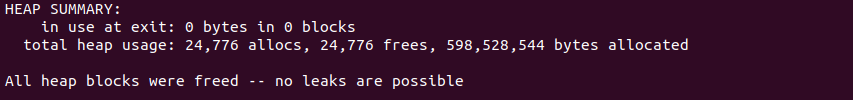
\includegraphics[scale=0.40]{memoryleaks.png}
    \caption{Verificação da libertação de memória.}
    \label{fig:memoryleaks}
	\end{figure}\\\\
De modo a mostrar a correta libertação de memória foi usado o \textit{Valgrind}, produzindo o resultado descrito na Figura~\ref{fig:memoryleaks}.\\\\
	
	\section{Alguns grafos}	
	\label{grafos}
	\begin{figure}[h!]
    \centering
    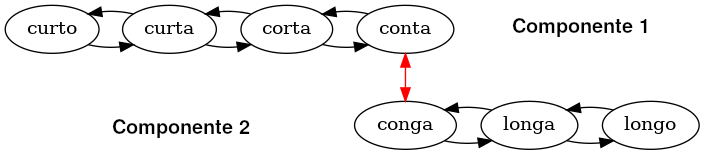
\includegraphics[scale=0.40]{uniao.png}
    \caption{União entre dois componentes conexos.}
	\end{figure}
\pagebreak
	\begin{figure}[h!]
    \centering
    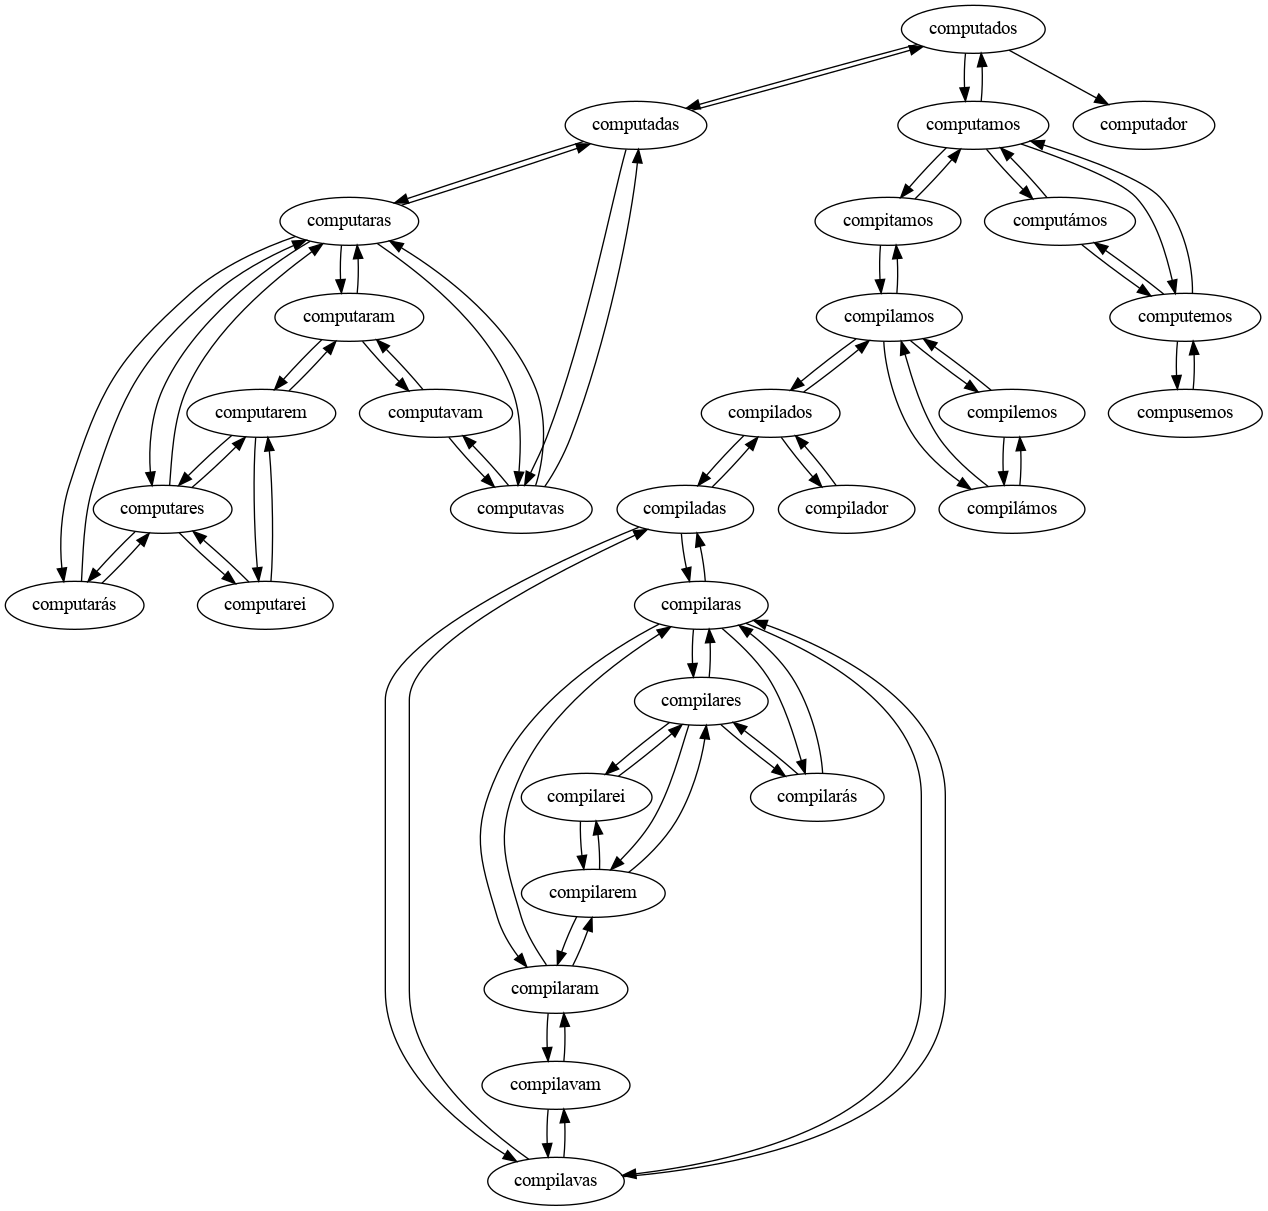
\includegraphics[scale=0.40]{graph1.png}
    \caption{Grafo do componente conexo da palavra "computador".}
	\end{figure}
\pagebreak
	\begin{figure}[h!]
    \centering
    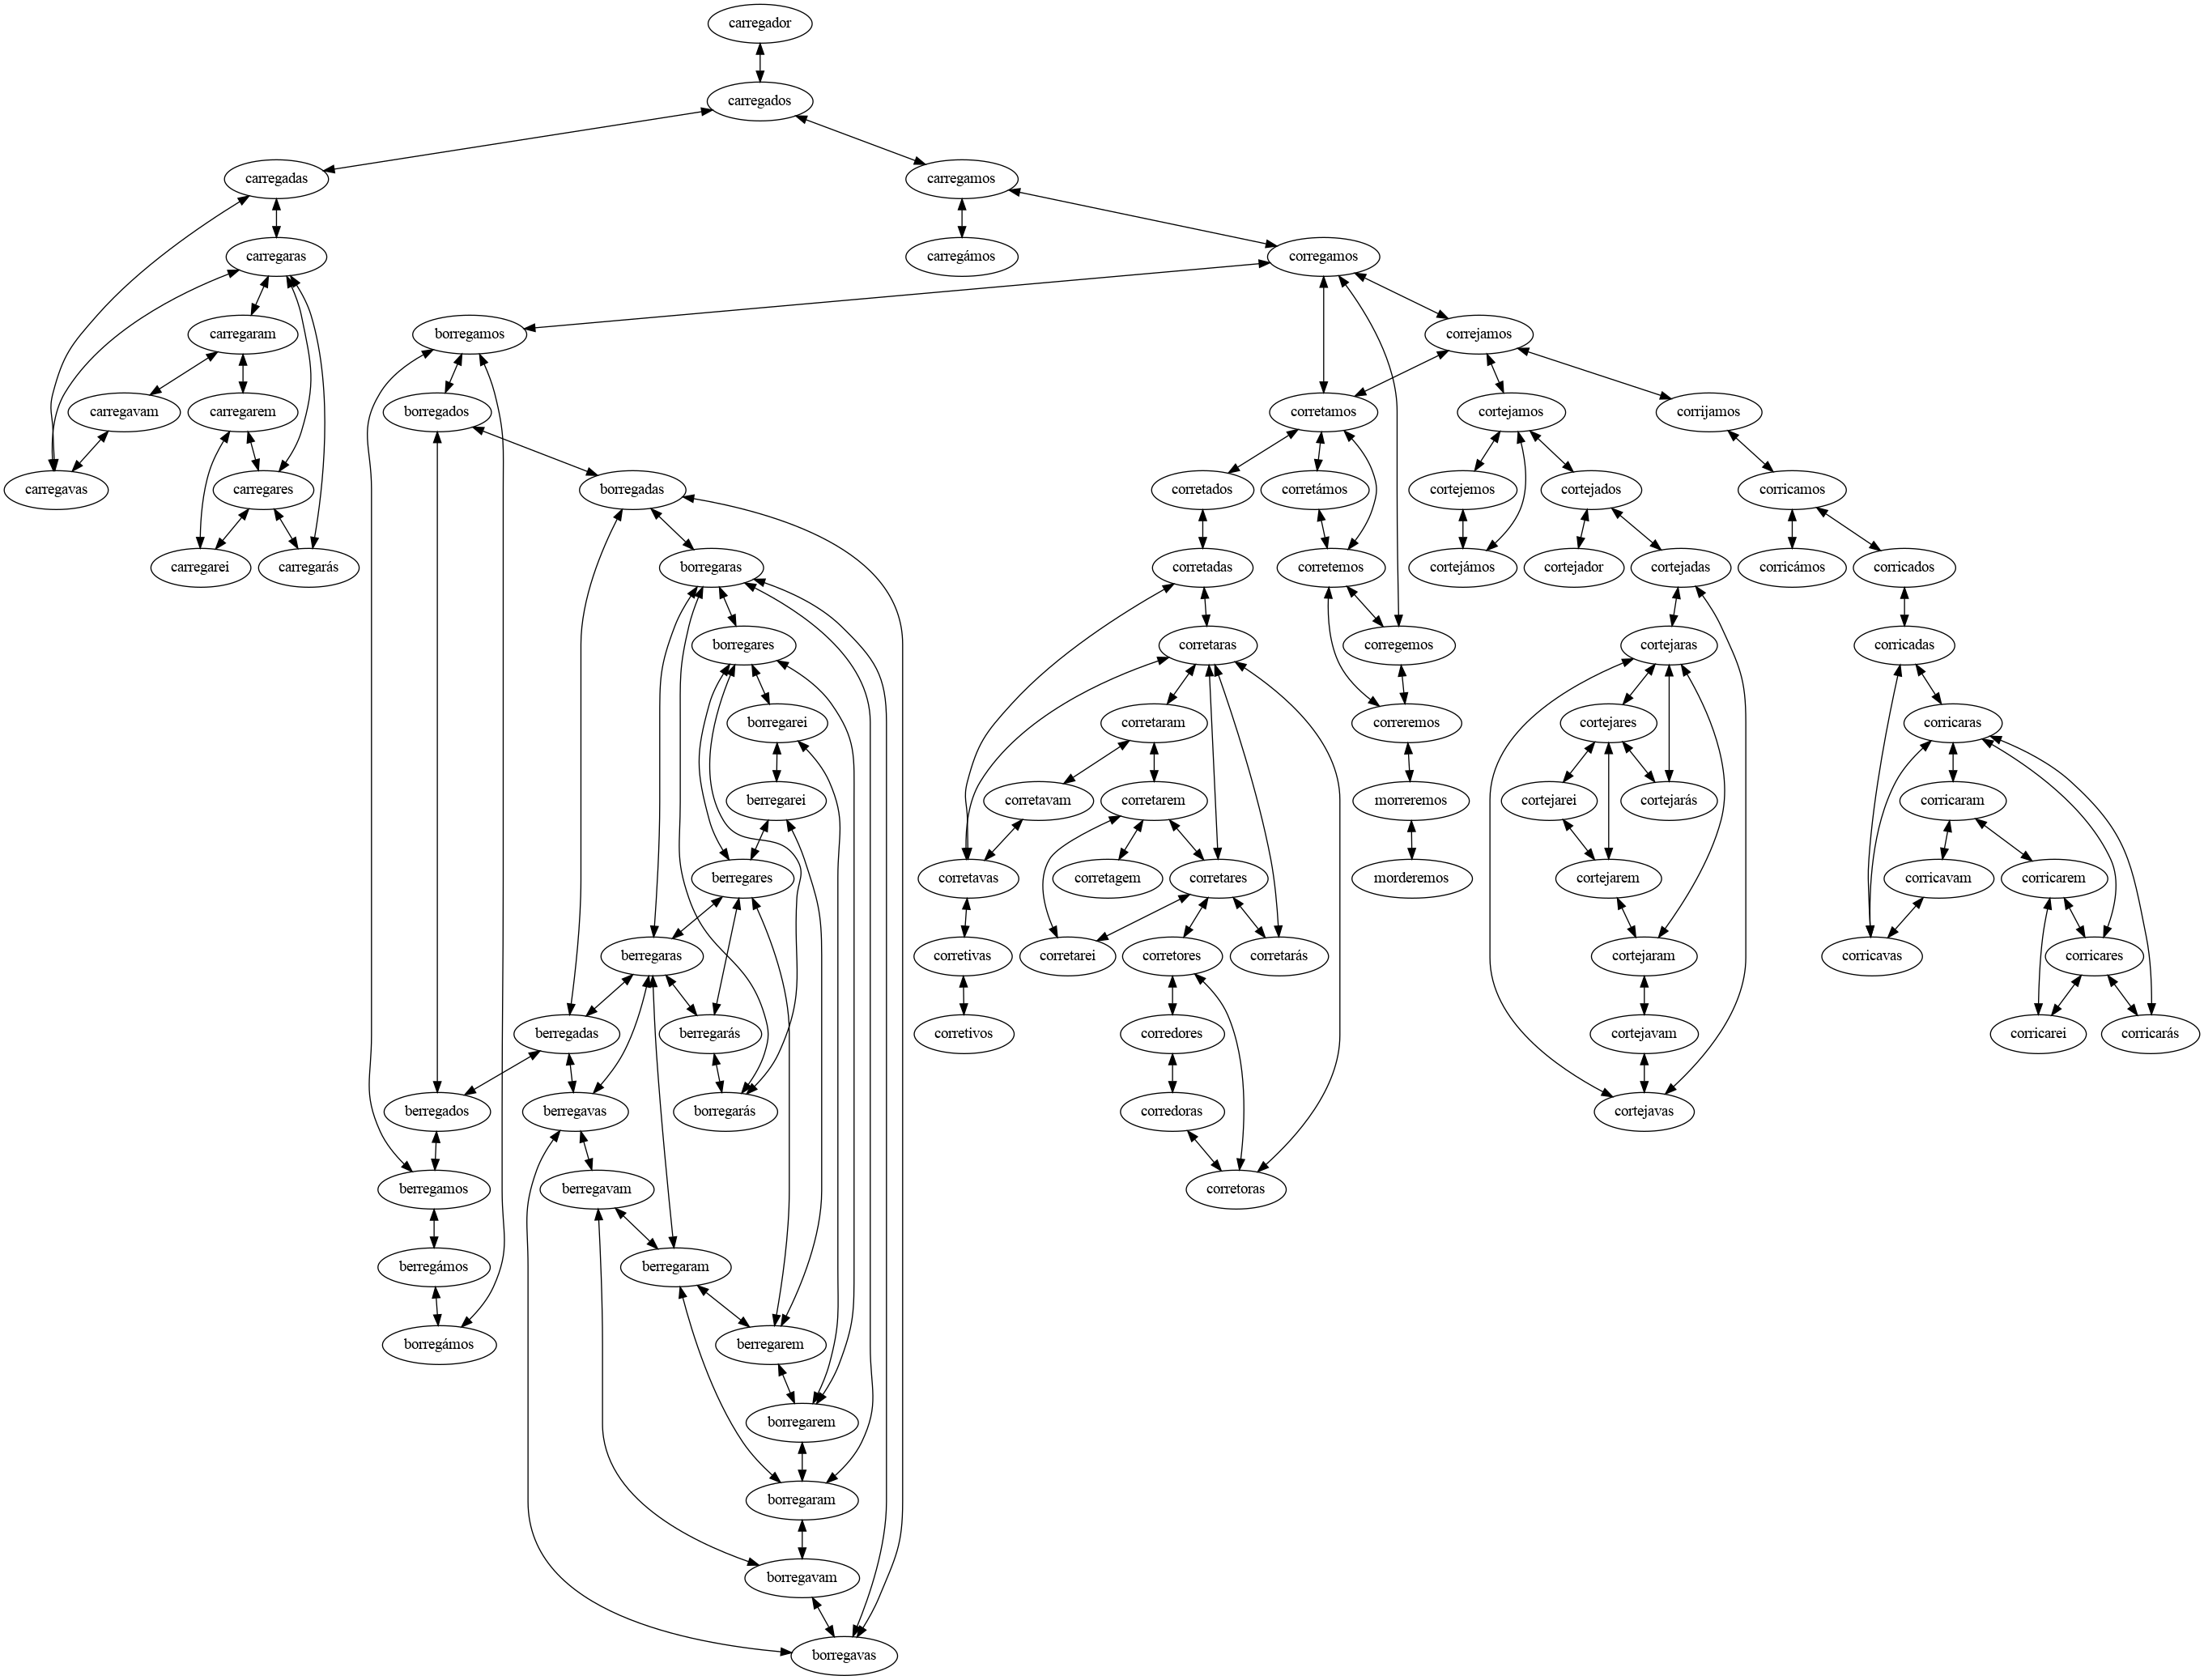
\includegraphics[scale=0.19]{graph.png}
    \caption{Grafo do componente conexo da palavra "carregador".}
	\end{figure}
\pagebreak
	\section{Curiosidades}
	\begin{figure}[h!]
    \centering
    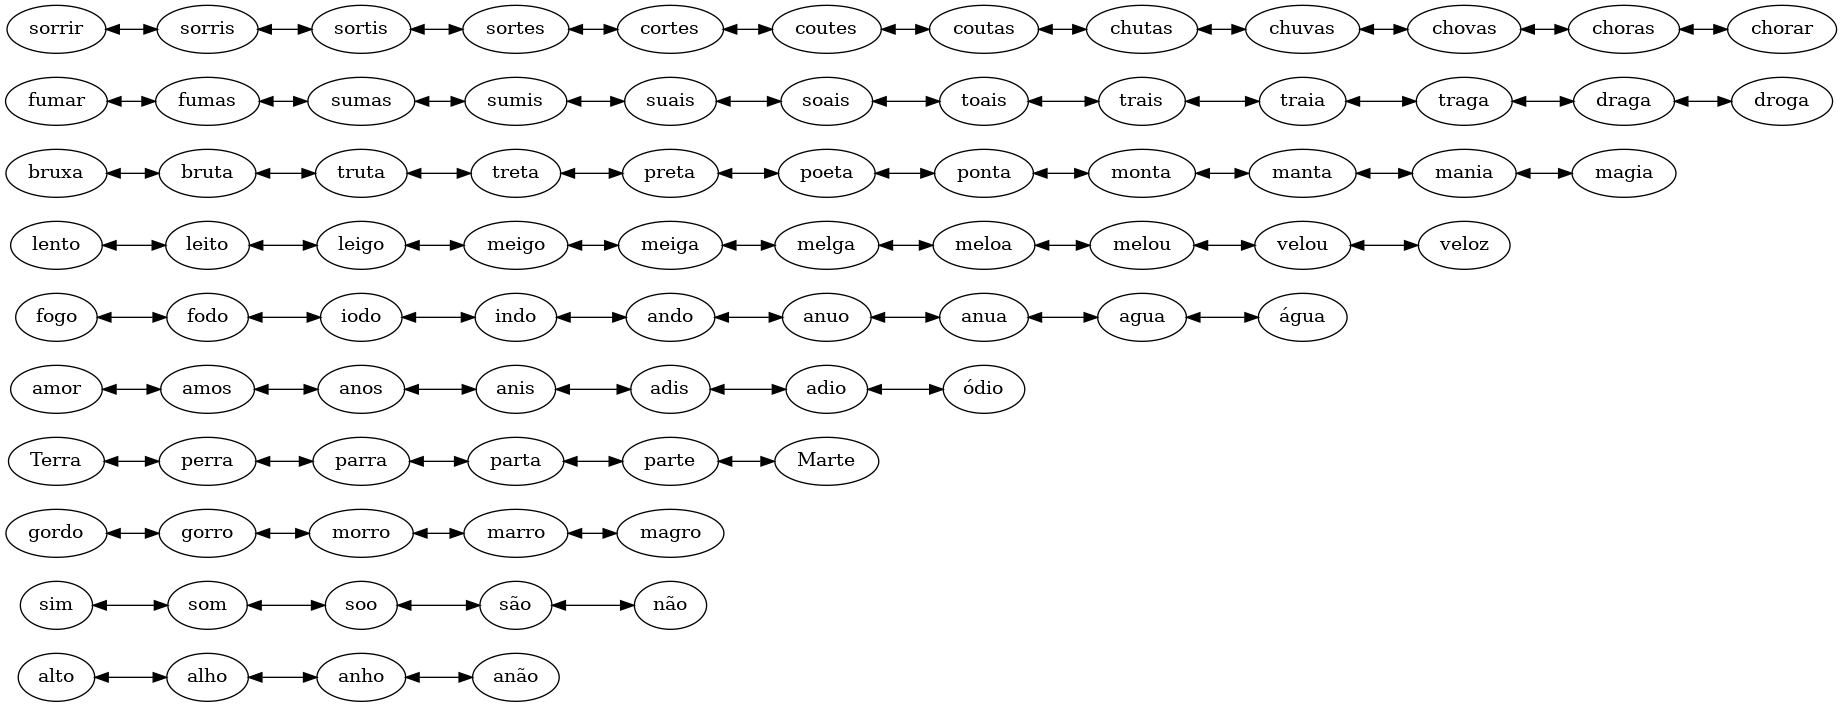
\includegraphics[scale=0.28]{curious.png}
    \caption{Exemplos de possíveis caminhos a serem testados.}
	\end{figure}
\chapter{Conclusão}
\label{conclusao}

Em suma, é possível concluir que este se trata de um trabalho em que a gestão correta de memória alocada se torna fundamental para uma boa execução do programa.\\
	Na solução apresentada, pode-se que concluir que a gestão da memória foi perfeita, uma vez que, com auxílio do Valgrind, se pode observar que não ocorreu qualquer \textit{memory leak}.\\
	Através do histograma apresentado, é possível concluir que a distribuição da hash table foi consistente e homogénea, detectando-se apenas um local com maior densidade de informação em relação aos restantes.\\
	Relativamente aos objetivos propostos, estes foram todos cumpridos e a sua execução não apresenta quaisquer problemas.

\begin{thebibliography}{9}
\vspace{5mm} %5mm vertical space

\bibitem{lecturenotes}
\textit{SILVA, Tomás Oliveira e. \textbf{Lecture notes}: Algorithms and Data Structures (AED — Algoritmos e Estruturas de Dados) LEC, LEI, LECI, 2022/2023.}
\bibitem{essentialInfo}
\textit{Robert Sedgewick, Kevin Wayne - Algorithms, 4th Edition\_ Essential Information about Algorithms and Data Structures-Addison-Wesley (2011)}
\bibitem{practicalprogramming}
\textit{Bruce Eckel, Chuck Allison - Thinking in C++, Volume 2\_ Practical Programming -Prentice Hall (2003)}
\bibitem{activelearning}
\textit{Jeffrey J. McConnell - Analysis of Algorithms\_ An Active Learning Approach-Jones & Bartlett Publishers (2001)}
\bibitem{graphcvizlink}
\textit{https://graphviz.org/} 
\bibitem{matlablink}
\textit{https://www.mathworks.com/products/matlab.html} 
\bibitem{octavelink}
\textit{https://octave.org/} 


\end{thebibliography}

\end{document}

